\documentclass[journal,compsoc, 10pt, draftclsnofoot, onecolumn]{IEEEtran}

\usepackage{graphicx}
\usepackage{amssymb}
\usepackage{amsmath}
\usepackage{amsthm}
\usepackage{tabularx}
\usepackage{graphicx}

\newcommand{\subparagraph}{}
\usepackage{titlesec}

\usepackage{alltt}
\usepackage{float}
\usepackage{color}
\usepackage{url}

\usepackage{balance}
\usepackage[TABBOTCAP, tight]{subfigure}
\usepackage{enumitem}
\usepackage{pstricks, pst-node}

\usepackage{cite}
\usepackage{listings}
\usepackage{placeins}

\usepackage[margin=0.75in]{geometry}
\geometry{textheight=8.5in, textwidth=6in}

\renewcommand{\familydefault}{\sfdefault}

\newlength\tindent
\setlength{\tindent}{\parindent}
\setlength{\parindent}{0pt}
\renewcommand{\indent}{\hspace*{\tindent}}

\newcommand{\cred}[1]{{\color{red}#1}}
\newcommand{\cblue}[1]{{\color{blue}#1}}

\newcommand{\namesigdate}[2][6cm]{%
  \begin{tabular}{@{}p{#1}@{}}
    #2 \\[0.5\normalbaselineskip] \hrule \\[0.pt]
    {\small \vspace{-3em} \textit{Signature}} \\[0.5\normalbaselineskip] \hrule \\[0pt]
    {\small \vspace{-3em}\textit{Date}}
  \end{tabular}
}


\usepackage{hyperref}
\usepackage{geometry}

\lstset{
language=C,
basicstyle=\ttfamily,
commentstyle=\color{blue},
numberstyle=\color{red},
stringstyle=\color{orange}
}

\def\nameD{Devin Foulger}
\def\nameH{Hector Trujillo}
\def\nameB{Bryan Liauw}

\usepackage{fancyvrb}
\usepackage{color}
\usepackage[latin1]{inputenc}


\makeatletter
\def\PY@reset{\let\PY@it=\relax \let\PY@bf=\relax%
    \let\PY@ul=\relax \let\PY@tc=\relax%
    \let\PY@bc=\relax \let\PY@ff=\relax}
\def\PY@tok#1{\csname PY@tok@#1\endcsname}
\def\PY@toks#1+{\ifx\relax#1\empty\else%
    \PY@tok{#1}\expandafter\PY@toks\fi}
\def\PY@do#1{\PY@bc{\PY@tc{\PY@ul{%
    \PY@it{\PY@bf{\PY@ff{#1}}}}}}}
\def\PY#1#2{\PY@reset\PY@toks#1+\relax+\PY@do{#2}}

\expandafter\def\csname PY@tok@gd\endcsname{\def\PY@tc##1{\textcolor[rgb]{0.63,0.00,0.00}{##1}}}
\expandafter\def\csname PY@tok@gu\endcsname{\let\PY@bf=\textbf\def\PY@tc##1{\textcolor[rgb]{0.50,0.00,0.50}{##1}}}
\expandafter\def\csname PY@tok@gt\endcsname{\def\PY@tc##1{\textcolor[rgb]{0.00,0.25,0.82}{##1}}}
\expandafter\def\csname PY@tok@gs\endcsname{\let\PY@bf=\textbf}
\expandafter\def\csname PY@tok@gr\endcsname{\def\PY@tc##1{\textcolor[rgb]{1.00,0.00,0.00}{##1}}}
\expandafter\def\csname PY@tok@cm\endcsname{\let\PY@it=\textit\def\PY@tc##1{\textcolor[rgb]{0.25,0.50,0.50}{##1}}}
\expandafter\def\csname PY@tok@vg\endcsname{\def\PY@tc##1{\textcolor[rgb]{0.10,0.09,0.49}{##1}}}
\expandafter\def\csname PY@tok@m\endcsname{\def\PY@tc##1{\textcolor[rgb]{0.40,0.40,0.40}{##1}}}
\expandafter\def\csname PY@tok@mh\endcsname{\def\PY@tc##1{\textcolor[rgb]{0.40,0.40,0.40}{##1}}}
\expandafter\def\csname PY@tok@go\endcsname{\def\PY@tc##1{\textcolor[rgb]{0.50,0.50,0.50}{##1}}}
\expandafter\def\csname PY@tok@ge\endcsname{\let\PY@it=\textit}
\expandafter\def\csname PY@tok@vc\endcsname{\def\PY@tc##1{\textcolor[rgb]{0.10,0.09,0.49}{##1}}}
\expandafter\def\csname PY@tok@il\endcsname{\def\PY@tc##1{\textcolor[rgb]{0.40,0.40,0.40}{##1}}}
\expandafter\def\csname PY@tok@cs\endcsname{\let\PY@it=\textit\def\PY@tc##1{\textcolor[rgb]{0.25,0.50,0.50}{##1}}}
\expandafter\def\csname PY@tok@cp\endcsname{\def\PY@tc##1{\textcolor[rgb]{0.74,0.48,0.00}{##1}}}
\expandafter\def\csname PY@tok@gi\endcsname{\def\PY@tc##1{\textcolor[rgb]{0.00,0.63,0.00}{##1}}}
\expandafter\def\csname PY@tok@gh\endcsname{\let\PY@bf=\textbf\def\PY@tc##1{\textcolor[rgb]{0.00,0.00,0.50}{##1}}}
\expandafter\def\csname PY@tok@ni\endcsname{\let\PY@bf=\textbf\def\PY@tc##1{\textcolor[rgb]{0.60,0.60,0.60}{##1}}}
\expandafter\def\csname PY@tok@nl\endcsname{\def\PY@tc##1{\textcolor[rgb]{0.63,0.63,0.00}{##1}}}
\expandafter\def\csname PY@tok@nn\endcsname{\let\PY@bf=\textbf\def\PY@tc##1{\textcolor[rgb]{0.00,0.00,1.00}{##1}}}
\expandafter\def\csname PY@tok@no\endcsname{\def\PY@tc##1{\textcolor[rgb]{0.53,0.00,0.00}{##1}}}
\expandafter\def\csname PY@tok@na\endcsname{\def\PY@tc##1{\textcolor[rgb]{0.49,0.56,0.16}{##1}}}
\expandafter\def\csname PY@tok@nb\endcsname{\def\PY@tc##1{\textcolor[rgb]{0.00,0.50,0.00}{##1}}}
\expandafter\def\csname PY@tok@nc\endcsname{\let\PY@bf=\textbf\def\PY@tc##1{\textcolor[rgb]{0.00,0.00,1.00}{##1}}}
\expandafter\def\csname PY@tok@nd\endcsname{\def\PY@tc##1{\textcolor[rgb]{0.67,0.13,1.00}{##1}}}
\expandafter\def\csname PY@tok@ne\endcsname{\let\PY@bf=\textbf\def\PY@tc##1{\textcolor[rgb]{0.82,0.25,0.23}{##1}}}
\expandafter\def\csname PY@tok@nf\endcsname{\def\PY@tc##1{\textcolor[rgb]{0.00,0.00,1.00}{##1}}}
\expandafter\def\csname PY@tok@si\endcsname{\let\PY@bf=\textbf\def\PY@tc##1{\textcolor[rgb]{0.73,0.40,0.53}{##1}}}
\expandafter\def\csname PY@tok@s2\endcsname{\def\PY@tc##1{\textcolor[rgb]{0.73,0.13,0.13}{##1}}}
\expandafter\def\csname PY@tok@vi\endcsname{\def\PY@tc##1{\textcolor[rgb]{0.10,0.09,0.49}{##1}}}
\expandafter\def\csname PY@tok@nt\endcsname{\let\PY@bf=\textbf\def\PY@tc##1{\textcolor[rgb]{0.00,0.50,0.00}{##1}}}
\expandafter\def\csname PY@tok@nv\endcsname{\def\PY@tc##1{\textcolor[rgb]{0.10,0.09,0.49}{##1}}}
\expandafter\def\csname PY@tok@s1\endcsname{\def\PY@tc##1{\textcolor[rgb]{0.73,0.13,0.13}{##1}}}
\expandafter\def\csname PY@tok@sh\endcsname{\def\PY@tc##1{\textcolor[rgb]{0.73,0.13,0.13}{##1}}}
\expandafter\def\csname PY@tok@sc\endcsname{\def\PY@tc##1{\textcolor[rgb]{0.73,0.13,0.13}{##1}}}
\expandafter\def\csname PY@tok@sx\endcsname{\def\PY@tc##1{\textcolor[rgb]{0.00,0.50,0.00}{##1}}}
\expandafter\def\csname PY@tok@bp\endcsname{\def\PY@tc##1{\textcolor[rgb]{0.00,0.50,0.00}{##1}}}
\expandafter\def\csname PY@tok@c1\endcsname{\let\PY@it=\textit\def\PY@tc##1{\textcolor[rgb]{0.25,0.50,0.50}{##1}}}
\expandafter\def\csname PY@tok@kc\endcsname{\let\PY@bf=\textbf\def\PY@tc##1{\textcolor[rgb]{0.00,0.50,0.00}{##1}}}
\expandafter\def\csname PY@tok@c\endcsname{\let\PY@it=\textit\def\PY@tc##1{\textcolor[rgb]{0.25,0.50,0.50}{##1}}}
\expandafter\def\csname PY@tok@mf\endcsname{\def\PY@tc##1{\textcolor[rgb]{0.40,0.40,0.40}{##1}}}
\expandafter\def\csname PY@tok@err\endcsname{\def\PY@bc##1{\setlength{\fboxsep}{0pt}\fcolorbox[rgb]{1.00,0.00,0.00}{1,1,1}{\strut ##1}}}
\expandafter\def\csname PY@tok@kd\endcsname{\let\PY@bf=\textbf\def\PY@tc##1{\textcolor[rgb]{0.00,0.50,0.00}{##1}}}
\expandafter\def\csname PY@tok@ss\endcsname{\def\PY@tc##1{\textcolor[rgb]{0.10,0.09,0.49}{##1}}}
\expandafter\def\csname PY@tok@sr\endcsname{\def\PY@tc##1{\textcolor[rgb]{0.73,0.40,0.53}{##1}}}
\expandafter\def\csname PY@tok@mo\endcsname{\def\PY@tc##1{\textcolor[rgb]{0.40,0.40,0.40}{##1}}}
\expandafter\def\csname PY@tok@kn\endcsname{\let\PY@bf=\textbf\def\PY@tc##1{\textcolor[rgb]{0.00,0.50,0.00}{##1}}}
\expandafter\def\csname PY@tok@mi\endcsname{\def\PY@tc##1{\textcolor[rgb]{0.40,0.40,0.40}{##1}}}
\expandafter\def\csname PY@tok@gp\endcsname{\let\PY@bf=\textbf\def\PY@tc##1{\textcolor[rgb]{0.00,0.00,0.50}{##1}}}
\expandafter\def\csname PY@tok@o\endcsname{\def\PY@tc##1{\textcolor[rgb]{0.40,0.40,0.40}{##1}}}
\expandafter\def\csname PY@tok@kr\endcsname{\let\PY@bf=\textbf\def\PY@tc##1{\textcolor[rgb]{0.00,0.50,0.00}{##1}}}
\expandafter\def\csname PY@tok@s\endcsname{\def\PY@tc##1{\textcolor[rgb]{0.73,0.13,0.13}{##1}}}
\expandafter\def\csname PY@tok@kp\endcsname{\def\PY@tc##1{\textcolor[rgb]{0.00,0.50,0.00}{##1}}}
\expandafter\def\csname PY@tok@w\endcsname{\def\PY@tc##1{\textcolor[rgb]{0.73,0.73,0.73}{##1}}}
\expandafter\def\csname PY@tok@kt\endcsname{\def\PY@tc##1{\textcolor[rgb]{0.69,0.00,0.25}{##1}}}
\expandafter\def\csname PY@tok@ow\endcsname{\let\PY@bf=\textbf\def\PY@tc##1{\textcolor[rgb]{0.67,0.13,1.00}{##1}}}
\expandafter\def\csname PY@tok@sb\endcsname{\def\PY@tc##1{\textcolor[rgb]{0.73,0.13,0.13}{##1}}}
\expandafter\def\csname PY@tok@k\endcsname{\let\PY@bf=\textbf\def\PY@tc##1{\textcolor[rgb]{0.00,0.50,0.00}{##1}}}
\expandafter\def\csname PY@tok@se\endcsname{\let\PY@bf=\textbf\def\PY@tc##1{\textcolor[rgb]{0.73,0.40,0.13}{##1}}}
\expandafter\def\csname PY@tok@sd\endcsname{\let\PY@it=\textit\def\PY@tc##1{\textcolor[rgb]{0.73,0.13,0.13}{##1}}}

\def\PYZbs{\char`\\}
\def\PYZus{\char`\_}
\def\PYZob{\char`\{}
\def\PYZcb{\char`\}}
\def\PYZca{\char`\^}
\def\PYZam{\char`\&}
\def\PYZlt{\char`\<}
\def\PYZgt{\char`\>}
\def\PYZsh{\char`\#}
\def\PYZpc{\char`\%}
\def\PYZdl{\char`\$}
\def\PYZti{\char`\~}
% for compatibility with earlier versions
\def\PYZat{@}
\def\PYZlb{[}
\def\PYZrb{]}
\makeatother


\hypersetup {
        colorlinks = true,
        urlcolor = black,
        linkcolor = black,
        pdfauthor = {\nameD\nameH\nameB},
        pdfkeywords = {},
        pdfsubject = {},
        pdfpagemode = UseNone
}

\titleformat{\section}
	{\normalfont\fontsize{15}{10}\bfseries}{\thesection}{1em}{}
\titleformat{\subsection}
	{\normalfont\fontsize{12}{15}\bfseries}{\thesubsection}{1em}{}
\titleformat{\subsubsection}
	{\normalfont\fontsize{12}{15}\bfseries}{\thesubsubsection}{1em}{}

\begin{document}

\title{\vspace{20em}Winterl Progress Report \\{\vspace{-1ex}\huge UniversityGear} \\
{\large \today}}
\author{\vspace{10ex}Devin Foulger \\{\vspace{-1ex}Hector Trujillo}
\\{\vspace{-1ex}Bryan Liauw}}

\begin{titlepage}

\maketitle
\thispagestyle{empty}

\begin{abstract}
This document will recap what we have done over the term and will describe 
what we plan to do in the following year. It will go into detail about the goals 
we have set and how we plan to accomplish them. It will also include a summary 
of the project status as it is now. It will also include a retrospective of what 
has happened throughout the term.
\end{abstract}

\end{titlepage}

\tableofcontents

\section{Introduction}
Throughout the term, we have been able to accomplish and learn a lot. We were 
able to design an application that will help people purchase college merchandise. 
We were able to come up with requirements and analyze the situation in a 
meaningful way. The team also analyzed many different technologies that we 
will be using to complete the project. 

\section{Project goals and recap}
The goal of the project is to build an Android application that will allow users 
to purchase college related merchandise. This means that users will be able to 
search for many items depending a lot of user provided information. They can 
search for specific schools and their colors as well as condition of item, or 
the price. We also set out to accomplish how to create documents in which we 
could effectively describe our project. \newline

Here our recaps from each term for each week.

\subsection{Fall Term}
\textbf{Week 2}\newline
During week 2, our group had just been in contact with our client, Luther. We 
discussed what was expected of the project and what eBay wanted. With this 
knowledge, we began work on our problem statement. This document outlined 
what was to be expected from the application that we would be developing. The 
team also set up a GitHub repo to hold all our documents and code. \newline

\textbf{Week 3}\newline
We completed our problem statement during week 3. After many emails with our 
client, we came to an agreement with the problem statement.  \newline

\textbf{Week 4}\newline
During week 4, we had began to make plans on what needed to be revised in the 
problem statement. The team had also created developer accounts on the eBay 
website and began looking at the APIs we would be using. We had also received 
a small rundown on what requirements will need to be met. Finally, we also began 
the weekly meetings with our TA.\newline

\textbf{Week 5}\newline
This week, we worked towards completing our requirements document. We had 
figured out what would need to be accomplished. Our client had also provided us 
with a mock up of what our application could look like. This helped with the 
creation of what requirements must be met.\newline

\textbf{Week 6}\newline
Over the course of week 6, the team accomplished a lot. We finished our 
requirements document and met with our client in Portland. After meeting with 
the team at eBay, it really felt like they wanted us to succeed. They helped us 
to better define the requirements that needed to be completed.\newline

\textbf{Week 7}\newline
During week 7, we began work on the tech review. We had split the requirements 
into three major parts: Searching and gathering data, UI and presenting data, and 
purchasing the items. After that, each team member focused on the parts that they 
had been assigned. \newline

\textbf{Week 8}\newline
Over week 8, the team did a mock design of what the application would look like. 
This was the beginning of the design document. Each member had also completed 
their part of the tech review. The review featured many different technologies that 
we would be using, discussing the benefits of each one. \newline

\textbf{Week 9}\newline
Large portions of the design document were completed over week 9. The group 
created a UML to demonstrate what classes might be used during development. 
\newline

\textbf{Week 10}\newline
The final week of the term, we completed our design document. However, we still 
needed to begin work on the fall progress report. \newline

Overall, we set out to accomplish many goals over the term. The end result of 
each of our documents provides us with a good start for development. 

\subsection{Winter Term}
\textbf{Week 1}\newline
During week 1, we talked about when we were going to meet to do some paired 
programming. We also uploaded our blank Android project to GitHub to get 
started. We also spent the time earlier during the term and the break learning 
how most other website, such as Google and Yahoo, employ their search 
function, which we ideally want to mimic. However, it turns out Google, 
which is the benchmark of search engines, employs a Levenshtein Distance
 method that is used alongside an artificial machine learning that takes in 
what people often search as probability. This advanced method is not viable 
for us because we would not have as much traffic, so we decided to stick with 
Levenshtein Distance only. \newline

\textbf{Week 2}\newline
This week we accomplished creating our search activity, however the class does 
not currently work with eBay's APIs. Basically what we have done is a basic 
search function with a textbox that gets user input. We also have a radio button 
that virtually does nothing but pass in the string that it contains. The input that 
the users give does nothing yet. We have yet to integrate any functionality from 
the eBay API. However, the text box does have limited Levenshtein Distance 
feature, in that we do not have a lot of keywords that user's input can be 
changed to. This early version of Levenshtein Distance has a lot of bugs that 
happens because the toleration level for mistakes is too high, which we have 
corrected.  \newline

\textbf{Week 3}\newline
For this week, we were able to get eBay's search API integrated with our 
search class allowing for us to make searches.This is done through passing 
in a HTTP requests using an asynchronous task class that is integrated inside the 
activity. After this milestone, we can finally use the result from the search
 activity to start working on other activity. However, this API needed 
authentication, which we arbitrarily pass in. This is not viable for beta release 
since the authentication, which utilizes oAuth keys, changes every two days. 
The filters also pass in words instead of actually filtering. On top of that, we 
also started the list view activity and the item class. The item class will allow us to create 
items in any class. The list view allows us to view the items by using a recycler 
view.\newline

\textbf{Week 4}\newline
During week 4, we have been connecting everyone's pieces. This means that we 
can now go from searching to the list view correctly displaying search results. 
The list view correctly displays the title, image, and price of the item. The 
item class is also continually being added to, depending on what new variables
we will be needing. \newline

\textbf{Week 5}\newline
 We added secondary filter activity as well as a method that gives new oAuth 
token every time it is called. For now, a new oAuth token is going to be 
retrieved every time a search is being submitted. The filters now utilize the 
filter options provided by the eBay API such as the price range and item 
condition. We also provided item categories to limit the search for the user. 
We also changed some filter categories and how a search works. Now, 
prior to actually searching for the item, we asked the user for a particular 
school first. This is done through typing in the school name in the text box 
or pressing one or more of the toggle buttons provided and then pressing the 
next button. It will pass in the value as an extra message for intent. We have 
not given the ability to pass in both value from the text box and the toggle 
buttons because we feel that it is not necessary for the user to do. After 
going through selecting the school, we provide the user with a text box and 
several check boxes for user to limit their search. Submitting it will send the
 keywords and filters to eBay's server, which we will return the result afterwards. 
This process is from one of the examples that eBay actually provided us with. 


\section{Project status}
The design for our application, UniversityGear, has been fairly complete. We 
have detailed the functional requirements of our project. We have also completed 
a technology review in which we discovered what technologies would be the most 
efficient with our application. Last, we created a design document to detail how 
we were going to implement the technologies we have found into our application.
After many weeks of communication with our client, we have arrived at the 
development phase.\newline

We have developed over half of our application. So far, we have implemented the 
ability to search, view, and select single items. This alone is a large part of 
the project. In the coming weeks, users will be able to purchase items, as well 
as use several filters to find the items that they need. These classes we have 
created also interact with eBay's APIs. So far, we have used their Browse API, 
but now we are going to be using the Order API to allow users to purchase the 
items that they want. 

\subsection{Search Class Development}
The search class is the first activity that the users are greeted by. They will 
interact with this class first. as it is required to get any results. 
This search activity will also function as our home page which consists of a
simple design that contains a search text field and a search button. Once the 
user presses the search button, the Search Activity takes the input and 
searches' eBay's database for related items. We were also able to implement a 
progress bar that shows up when the user clicks on Submit and disappears when 
the search results are ready to be presented. This is important because it lets 
the user know that the application is processing the request. 

\subsection{Notification's Development}
Have implemented the Alert notification that lets the user know that their 
keyword/s did not return any results. This message is important because it 
lets the user know that the application is working as it should, and there 
were simply no items containing the keyword/s that they used.

\subsection{Item Class Development}
The item class is what allow us to build specific items or a list of items. 
First, the class will create a list of items that will be displayed to the 
user in a list item view. Once an item is selected from the list, the item 
class will build another single item, with much more information pertaining to 
the item selected. Development for this class is something that will be ongoing 
throughout the project. This is because more information may need to be grabbed 
depending on what kind of item is being selected. However, development was rather 
straight forwarded, as we grabbed the specific information we needed. \newline

It was important that this was one of the first classes that 
needed to be created. This is because other parts of the project will heavily 
depend upon this class. This class used the standard JSON methods that are 
present in Java. These tools allowed us to parse and gather the correct 
information that we needed. All of the data returned by eBay's APIs are in 
JSON format.  So far, the class will return many things like the items title, 
price, description, color, material, pattern, type, and category. 

\subsection{List View Development}
Successfully completed the presentation of the search results in a list view. 
This list view displays the item title, image, and item price for every image 
that is returned. The user is allowed to scroll through the different items 
until they find one that catches their attention. We also set up the 
"onClickListener" for each item so that when a user clicks on an item that they 
like, they are presented with more details on that specific item.


\subsection{Single Item Activity}
The single item activity class is what the users use to view the single item they 
have selected. This activity will display the pertinent information of an item, 
like its title, color, price, description, material, pattern, and any other item 
specific information. This class made use of eBay's Browse API. Specifically, it 
used the get item method, which retrieves data for a given item. 

This activity is started after a user selects a single item from the list view. From 
there, it passes in the item id to the single item activity. The single item 
activity then uses that item id in the eBay API. The API then returns a JSON file 
with all of the information on the item. When searching for things like mugs, it 
won't contain the same contents as a jacket would. A mug might only show the 
fields material, while a jacket could have a pattern and a material field. 
So the content displayed to the user is somewhat dynamic. \newline

The UI for the single item activity resembles the style of the eBay app.  The layout is rather 
simple and it is easy to follow. It is broken into several sections. The first 
section is the image, title, and price of the item. From there, we have the 
description and the purchase button. Then there is the about section. It contains 
the condition of the item, its quantity, category, brand, and other important 
information. The last section is the shipping and return info. This section states 
what kind of return policy the item has and how long a user will have to return the 
item. It also specifies who pays for returns on the item.\newline

\subsection{Location-based Recommendation}
An implementation that we would like to consider as a stretch goal is using 
Androids GPS to get user's location and give a list of recommended school 
based on this information. This could potentially increase the usability of our 
application. This might not be a hard method to implement as the location is 
mostly available in one of the Androids built-in function. The difficulty would 
lie in assigning the location to the schools. This would be time-consuming. 
Also, this function is definitely not a requirement so we can put this off.

\subsection{Utilizing Storage}
Storage is not fully utilized yet. Although this does not affect performance as 
much, we would like to increase the speed on how user will be able to search. 
While we have a storage method in the search activity, it is a stub currently 
and does nothing but saving what user has inputted. We need to be able to 
find a way to integrate this to either filter function or text box function. Also,
 we need to test the 

\subsection{Keyword Bank for Levenshtein Distance}
We would like to improve on is the Levenshtein Distance keywords list. For now, 
we have a limited list of keywords. This, while not essentially hindering usage of 
the app, limits a lot of what could potentially help user in the searches. Currently,
 our implementation relies on an array that consists of only several words. We would 
like to use an internal storage to store a list of keywords as well as school names.

\subsection{Bug Testing}
We also need to test this activity to ensure that it is bug-free. For now, we would 
want to try passing in empty string and making sure it will not crash. Another error 
we think might possibly happen is when we return to the previous activity. This will 
usually happen because the stack is not what we thought it is. This is one of the 
places where we think it is vulnerable.

\section{Impediments and solutions}
Over the course of the term, our team managed to avoid many impediments. However, 
we did need to revise our problem statement. In order to solve this, we re-wrote the 
problem statement with the revisions provided by the professors of the capstone 
class. \newline

Another problem is the design documents. The format that is required is not 
something we are familiar with. There is a lot of questions regarding what to 
put where. After looking at several examples, as well as asking people, 
we managed to get it done in the end.\newline

Initially, we had hoped to get started on the project during winter break. 
It proved difficult to find the energy to work on it after a grueling Fall 
term. Some of the items that we had hoped to accomplish during this time was 
to become familiar with eBay's APIs and how to use them. Another goal that we 
had for the break was to get familiar with the technology that we were going 
to be using to implement the list item view and the Android notification/alert 
systems. The failure to work on these goals during the break, didn't have a 
large impact on the project. The main consequence was that we had more work to 
do in a shorter period. Also, it did slow down development just a bit as we 
familiarized ourselves with the technologies being used, however we were able 
to recover from this slow start to get back on schedule.\newline

We have run into several problems trying to integrate the eBay API. We do not know 
exactly know what variable they want at first for authentication. Since they have two 
different oAuth keys, it turns out we were using the wrong oAuth key the whole time. 
Another problem is that we pass in an incorrect value due to our method of encoding. 
We thought the encoding would use a default encoding when the value is actually 
somewhat modified. We managed to solve both these problems by communicating 
with our clients. \newline

A problem that still remains unsolved is that one of our members broke his gradle build. 
This becomes a huge problem because he is unable to open changes that we made into 
his own computer, therefore relying on meetings to catch up with the rest of our work. 
However, despite this, he can work around it by working on one activity at a time. Since 
we have our meetings pretty frequently, we can rectify this pretty easily.

\section{Remaining Items}

\subsection{Item Filter Development}
One of the larger pieces that still needs to be developed is the implementation
 of the Search filters. These filters will help the user narrow down their 
search results to display items that are truly relevant to what they are 
looking for. For the alpha release we will have the front end complete. This 
will consist of having the filters available for the user to select, but the 
will not do anything until after the alpha release. 

\subsection{Internet Connectivity Verification}
Another small, but important item that still needs to be implemented is to 
have the application check to ensure an active internet connection. If the 
user does not have an active internet connection, we will display an alert 
stating that a connection to the internet is a requirement to using the 
application.  This will help in avoiding scenarios where the user tries to 
search for items, but nothing happens because they are not connected to the 
internet. 

\subsection{Purchase Class Development}
One of the larger classes, the purchase class, still needs to be developed before 
the end of the term. This class is what will allow users to purchase an item of their 
choice. In order to implement this class, we will need to use eBay's Order API. The 
Order API allows us to use guest checkout, meaning that any user will be able to 
use our app without a log in.

\subsection{Known Bugs}
Improve or fix the way images are being presented within the current list view 
results. There are certain items who's images are cropped out because they are 
either too big or are in portrait mode. Ensuring that the images fit into their 
intended area will be important so that the users can see the entire image and 
thus get a good idea of the product that is for sale. There is also a bug in 
the list view results display that we need to track down and fix. The bug 
results in images not displaying at all when the user is viewing the search 
results in a list view. However, the item displays as it should in the single 
item view. The part that makes it harder to identify is the fact that this bug 
is only present when working in the sandbox environment. When testing the 
application on eBay's production servers, the images display properly on both 
the list view and single item view. It could come down to being an issue with 
the data in eBay's sandbox environment. To determine this, we will need to do 
plenty of testing, and discuss with our client eBay potential causes for the 
different behavior in the different environments. 

\section{Project Images}
\begin{figure}[h]
This image demonstrates what is displayed to the user after they successfully 
complete a search. This will list all possible searches. Each item card will display 
the title, image and price. 
\centering
\caption{List view of items}
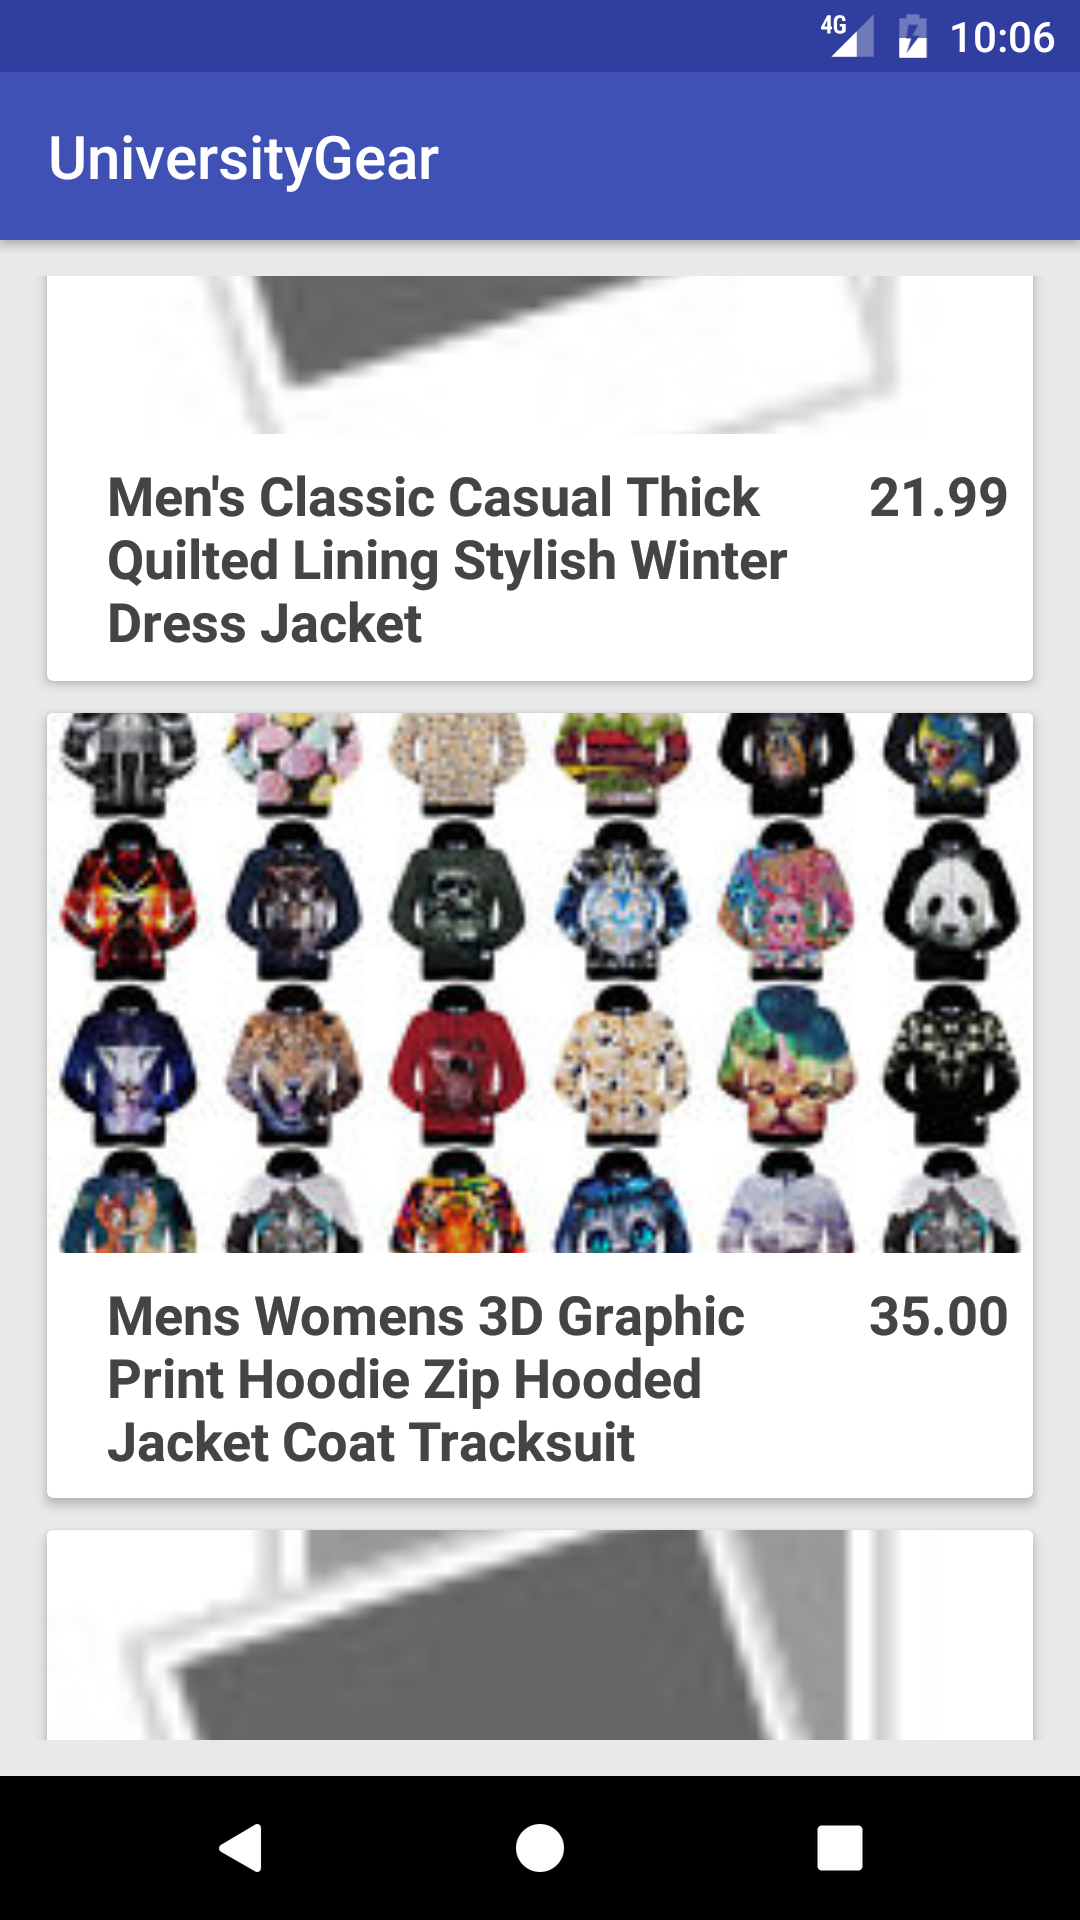
\includegraphics[scale=.2]{listview}
\end{figure}

\begin{figure}[t]
This is an image of what a single item would look like when being viewed. 
It contains the title, price, and other important information that pertains to 
the item.
\centering
\caption{Image of single item}
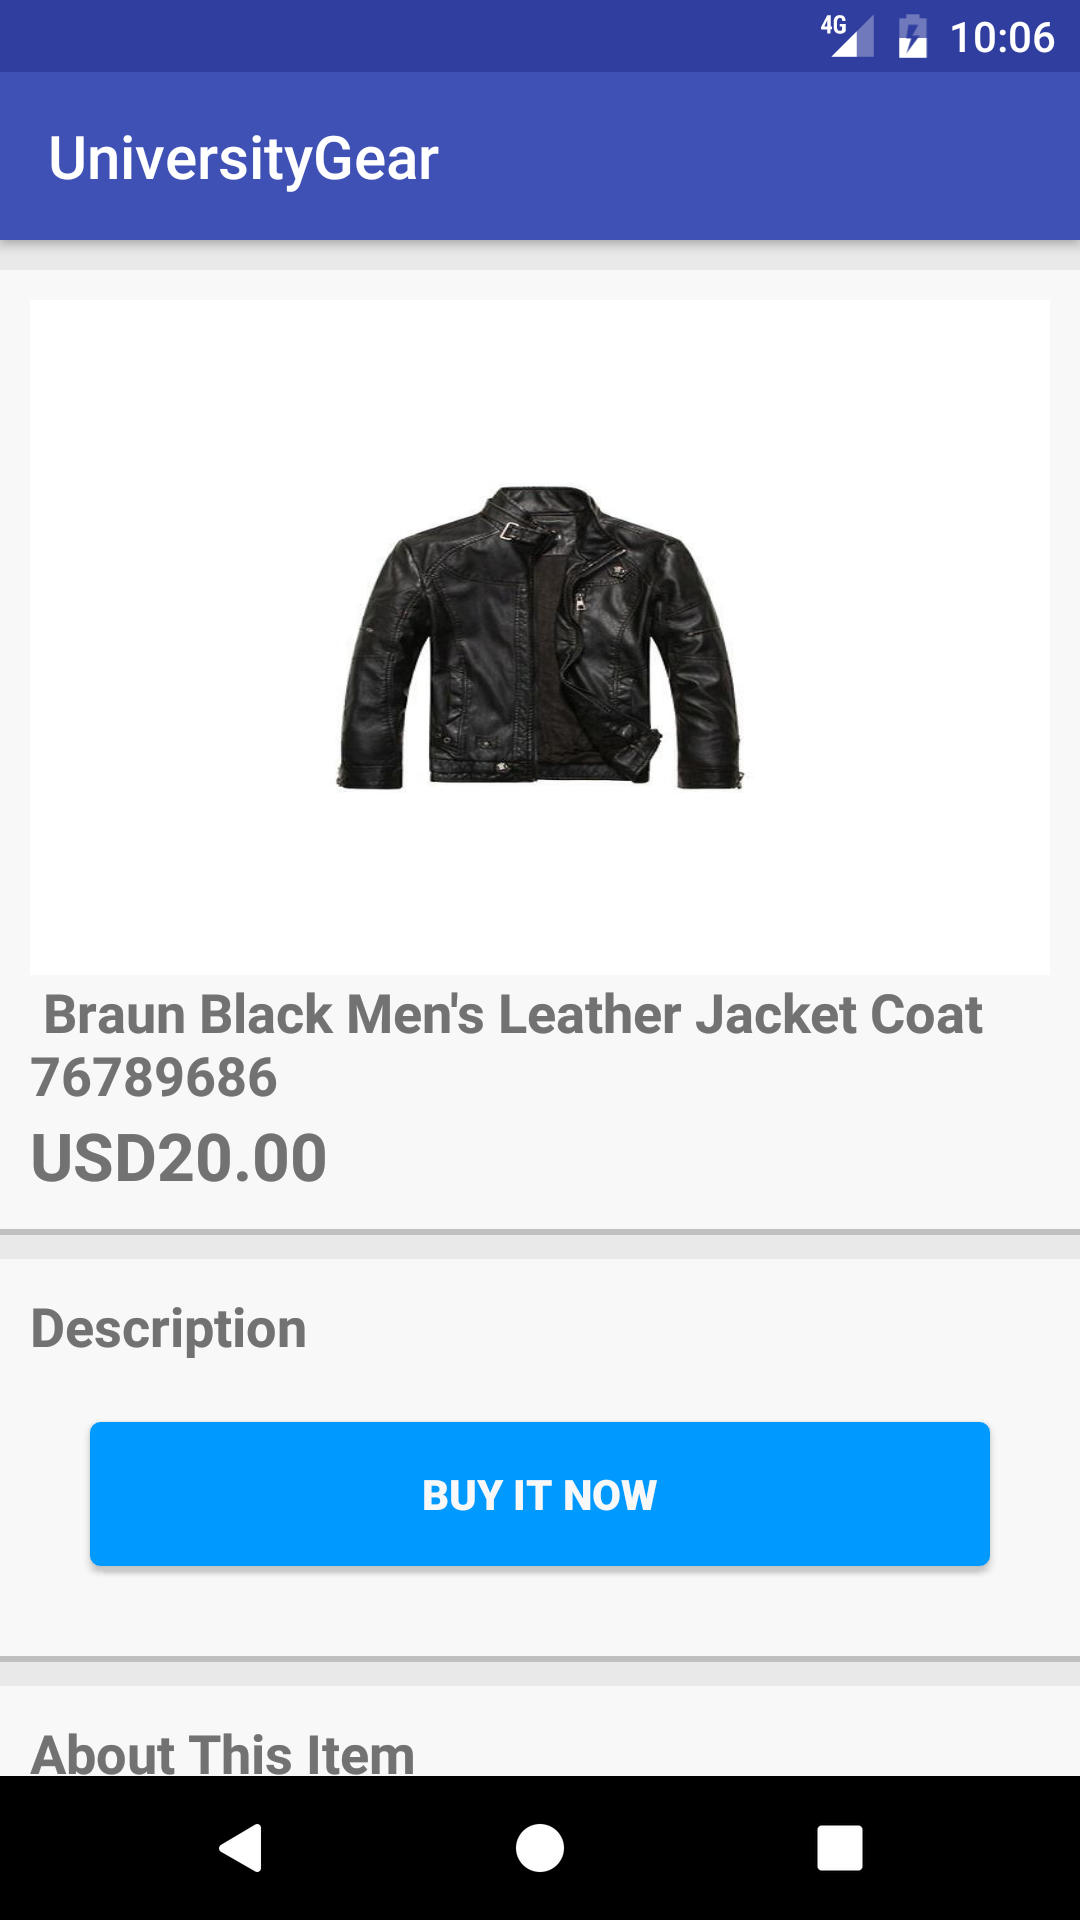
\includegraphics[scale=.2]{singleview1}
\end{figure}

\begin{figure}[t]
This is what the rest of the single item view would display to the user. It 
shows more details about the item as well as shipping and return info.
\centering
\caption{Item details of a single item}
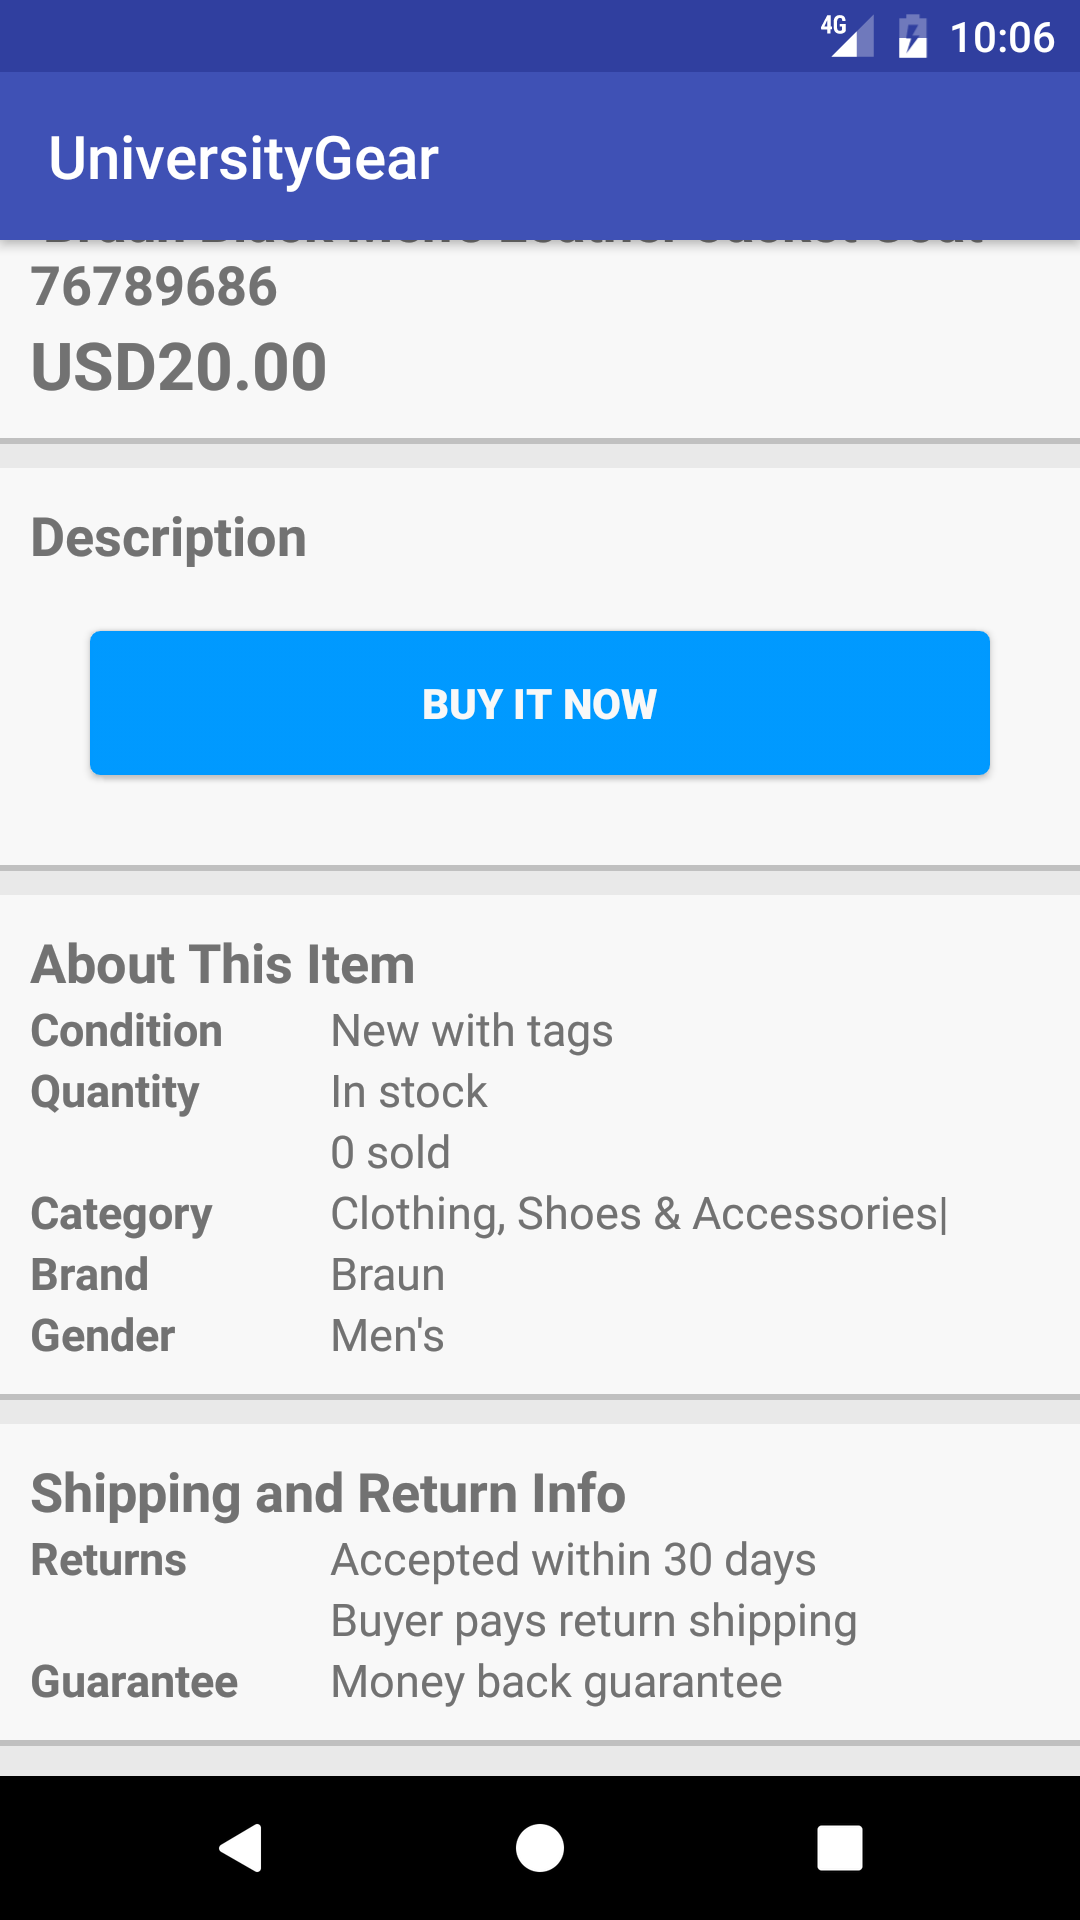
\includegraphics[scale=.2]{singleview2}
\end{figure}
\FloatBarrier

\section{Retrospective}

\begin{table}[!ht]
\centering
\caption{Retrospectives}
\label{my-label}
\begin{tabularx}{\textwidth}{X|X|X}
\hline
\textbf{Positives} & \textbf{Deltas} & \textbf{Actions} \\ \hline
Completed the problem statement                  &  Didn't meet the criteria                &Rewrote the report to define the problem better                 \\ \hline
Met with the client in Portland                  &     Could meet with clients more frequently            & Arrange more meetings on-line                 \\ \hline
Completed the requirements document                  & Not quantifying goals, spelling errors, and missing an abstract                & Proofreading it more and asking for more clarifications prior to submitting it                 \\ \hline
Completed the technology review                 & Writing could be improved                & Go to the Writing Center in order to see missed mistakes                 \\ \hline
Completed the design document                  & Can start earlier                 &Talk more to TA and instructor on clarifying some matters                  \\ \hline
\end{tabularx}
\end{table}

\FloatBarrier
\section{Conclusion}
During the course of the term we have learned many things. This includes items 
from different IEEE formats used in the real world to best practices when gathering 
project requirements. We also learned how to look at projects from the 10,000 
foot level instead of trying to focus on specific details. We will begin development 
on our project during winter term. However, we are hoping to make progress 
during winter break. Over half of winter term and we have already accomplished 
half of what we have set out to do. 

\end{document}